%%%%%%%%%%%%%%%%%%%%%%%%%%%%%%%%%%%%%%%%%%%%%%%%%%%%%%%%%%%%%
%% Begin exercise %%
%%%%%%%%%%%%%%%%%%%%%%%%%%%%%%%%%%%%%%%%%%%%%%%%%%%%%%%%%%%%%

\ex{Flyback converter /}

%%%%%%%%%%%%%%%%%%%%%%%%%%%%%%%%%%%%%%%%%%%%%%%%%%%%%%%%%%%%%
%% Task 1: Flyback converter %%
%%%%%%%%%%%%%%%%%%%%%%%%%%%%%%%%%%%%%%%%%%%%%%%%%%%%%%%%%%%%%
\task{Flyback converter}
A flyback converter with an input voltage range $U_\mathrm{1} = \SI{300}{\volt} \, \dots \, \SI{900}{\volt}$ is used to supply the control electronics of a frequency inverter. The converter delivers a rated output power of  $P_\mathrm{2} = \SI{30}{\watt}$ at a regulated (constant) output voltage of  $U_\mathrm{2} = \SI{15}{\volt}$. The flyback converter is operated in discontinuous current mode with a constant frequency of  $f_\mathrm{p} = \SI{500}{\kilo\hertz}$. The transformation ratio of the transformer is $N_\mathrm{1}/N_\mathrm{2}=60/12$, the inductance of the primary winding is $L_\mathrm{1} = \SI{760}{\micro\henry}$. The coupling between the primary and secondary windings is ideal. You can assume stationary operation for all calculations.

%%%%%%%%%%%%%%%%%%%%%%%%%%%%%%%%%%%%%%%%%%%%%%%%%%%%%%%%%%%%%%%%%%%%%%%
 % Flyback converter Schematic
%%%%%%%%%%%%%%%%%%%%%%%%%%%%%%%%%%%%%%%%%%%%%%%%%%%%%%%%%%%%%%%%%%%%%%%
           
           \begin{figure}[htb]
                \begin{center}
                    \begin{circuitikz}[european currents,european resistors,american inductors]
                    \draw (0.5,0) to [short] ++(0.5,0)
                    to [diode, l=$D$]  ++(1.0,0)
                    to [short, -o, i=$i_2(t)$] ++(1.0,0)
                    to [open, o-o, v = $\hspace{2cm}u_2(t)$, voltage = straight] ++(0,-2) coordinate (A)
                    (-0.5,0) to [short, -o, i_<=$i_1(t)$] ++(-1.5,0)
                    to [open, o-o, v_= $u_1(t)\hspace{0.75cm}$, voltage = straight] ++(0,-3.75) coordinate (B)
                    (-0.5,0) to [inductor, n=l1] ++(0,-2) 
                    to [Tnpn, n=npn1, mirror] ++(0,-1.75) coordinate (C)
                    (0.5,0) to [inductor, n=l2, mirror] ++(0,-2) coordinate (D)
                    (D) to [short, -o] (A)
                    (C) to [short, -o] (B);
                    \draw let \p1 = (npn1.B) in node[anchor=south] at (\x1,\y1) {$T$};
                    \path (l1.ul dot) node[circ]{}
                        (l2.ur dot) node[circ]{};
                    \draw (l1.midtap) node[left]{$N_1$}
                    (l2.midtap) node[right]{$N_2$};
                    \draw[double, double distance=3pt, thick] let \p1=(l1.core west), \p2=(l2.core east) in (\x1/2+\x2/2, \y1) -- (\x1/2+\x2/2, \y2);
                \end{circuitikz}
            \end{center}
                \caption{Flyback converter topology}
                \label{fig:flyback_converter_topology}
            \end{figure}
        

\begin{table}[ht]
    \centering  % Zentriert die Tabelle
    \begin{tabular}{llll}
        \toprule
        
        Input voltage: &  $U_{\mathrm{1}} = \SI{300}{\volt} \, \dots \, \SI{900}{\volt}$ & Output voltage: & $U_{\mathrm{2}} = \SI{15}{\volt}$ \\ 
        Output power: & $P_2 = \SI{30}{\watt}$  & Transformation ratio: & $N_\mathrm{1}/N_\mathrm{2}=60/12$ \\ 
        Inductance of the primary winding: & $L_\mathrm{1} = \SI{760}{\micro\henry}$ & Switching frequency: & $f_{\mathrm{s}} = \SI{50}{\kilo\hertz}$ \\ 
        \bottomrule
    \end{tabular}
    \caption{Parameters of the boost converter.}  % Beschriftung der Tabelle
    \label{table:ex04_Parameters of the circuit}
\end{table}

\subtask{The input voltage is $U_\mathrm{1}=\SI{760}{\volt}$ at rated power at the output. What is the peak value $\hat I_\mathrm{1}$ of the primary current $i_\mathrm{1}$? What is the peak value $\hat I_\mathrm{2}$ of the secundary current $i_\mathrm{2}$? Calculate the duty cycle of the transistor for this operating case.}

\begin{solutionblock}
To determine the current  $\hat I_\mathrm{1}$, the equation for determining the output power \eqref{eq:output power ex04} is primarily used. The unknown energy of the inductance of the primary winding side \eqref{eq:energy primary inductance ex04} is inserted into this equation.
\begin{equation}
    P_\mathrm{2} = W_\mathrm{L} f_\mathrm{p}, \label{eq:output power ex04}
\end{equation}

\begin{equation}
    W_\mathrm{L} = \frac{1}{2}L_\mathrm{1}\hat I_\mathrm{1}^2. \label{eq:energy primary inductance ex04}
\end{equation}
After substituting, you get this equation:
\begin{equation}
    P_\mathrm{2} = \frac{1}{2}L_\mathrm{1}\hat I_\mathrm{1}^2 f_\mathrm{p}.\label{eq:output power with IDach ex04}
\end{equation}
\eqref{eq:output power with IDach ex04} must be converted to $\hat I_\mathrm{1}$:
\begin{equation}
    \hat I_\mathrm{1} = \sqrt{\frac{2P_\mathrm{2}}{L_\mathrm{1}f_\mathrm{p}}}= \sqrt{\frac{2\cdot\SI{30}{\watt}}{\SI{760}{\micro\henry}\cdot\SI{50}{\kilo\hertz}}}=\SI{1.257}{\ampere}.
\end{equation}
In an ideal transformer, the energy is maintained between the primary and secondary sides (neglecting losses). To determine the peak value $\hat I_\mathrm{2}$, the known current $\hat I_\mathrm{1}$ and the number of turns of the primary and secondary side can be used. Because of this background, the following equation can be used:
\begin{equation}
    \hat I_\mathrm{2} = \hat I_\mathrm{1} \frac{N_\mathrm{1}}{N_\mathrm{2}} = \SI{1.257}{\ampere} \cdot \frac{60}{12} = \SI{6.28}{\ampere}.
\end{equation}
Because of CCM the duty cycle $D$ is expressed as
\begin{equation}
    \frac{U_2}{U_1} = \frac{D^2}{2} \frac{\Delta i_\mathrm{m,max}}{\overline{i}_2}. \label{eq:Duty cycle ex04}
\end{equation}
Because of the unknown $\Delta i_\mathrm{m,max}$ this value has to be calculate first as
\begin{equation}
    \Delta i_\mathrm{m,max}= \frac{T_\mathrm{s} \cdot U_1}{L} = \frac{\frac{1}{\SI{50}{\kilo\hertz}}\cdot \SI{760}{\volt}}{\SI{760}{\micro\henry}}=\SI{20}{\ampere}.
\end{equation}
Now $\Delta i_\mathrm{m,max}=\SI{20}{\ampere}$ can be used in \eqref{eq:Duty cycle ex04}:

\begin{equation}
    D = \sqrt{\frac{2U_2\overline{i}_2}{U_1\Delta i_\mathrm{m,max}}} = \sqrt{\frac{2\cdot \SI{15}{\volt}\cdot\SI{30}{\watt}}{\SI{760}{\volt}\cdot\SI{15}{\volt}\cdot\SI{20}{\ampere}}} = 0.063.
\end{equation}

\end{solutionblock}

\subtask{The input voltage is  $U_\mathrm{1}=\SI{382}{\volt}$ at nominal load. Calculate and sketch the following voltage and current curves for this operating case over one cycle period: $u_\mathrm{T}(t), u_\mathrm{s}(t), i_\mathrm{2}(t), i_\mathrm{1}(t)$ (Note: corresponds to the switch-on time of the transistor).}

\begin{solutionfigure}[htb]
    \centering
    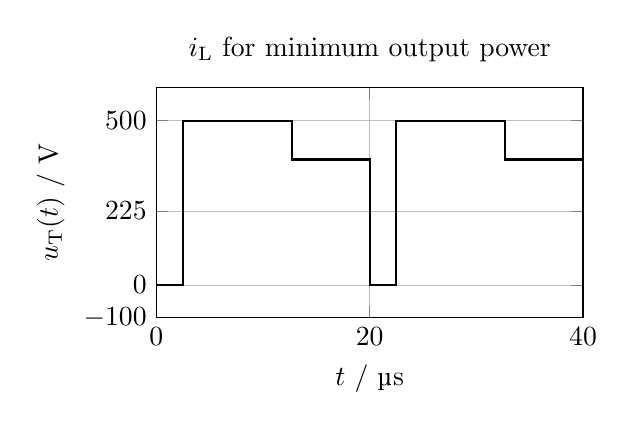
\begin{tikzpicture}
    \begin{axis}[
        width=7cm, height=4.5cm,
        grid=both,
        major grid style={line width=.2pt,draw=gray!50},
        minor grid style={line width=.1pt,draw=gray!20},
        xlabel={$t$ / µs},
        ylabel={$u_\mathrm{T}(t)$ / V},
        title={$i_\mathrm{L}$ for minimum output power},
        xmin=0, xmax=40,
        ymin=-100, ymax=600,
        xtick={0, 20, 40},
        ytick={-100, 0, 225, 500},
        ]
        % Einschaltverhalten graph
        \addplot[
            thick,
            mark=none,
            color=black,
        ] coordinates {
            (0,0) (2.5,0) (2.5, 500) (12.7, 500) (12.7, 382) (20, 382) (20, 0) (22.5, 0)(22.5, 500) (32.7, 500) (32.7, 382) (40, 382)
        };
    \end{axis}
    \end{tikzpicture} 
    \hspace{1cm} % Abstand zwischen den beiden Diagrammen
    \caption{Display of the voltage $u_\mathrm{T}(t)$.}
    \label{fig:voltageTransistorPeriodTask1}
    \end{solutionfigure}
\begin{solutionfigure}[htb]
    \centering
    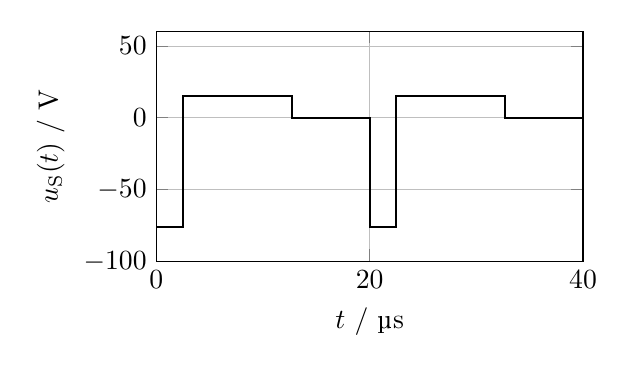
\begin{tikzpicture}
    \begin{axis}[
        width=7cm, height=4.5cm,
        grid=both,
        major grid style={line width=.2pt,draw=gray!50},
        minor grid style={line width=.1pt,draw=gray!20},
        xlabel={$t$ / µs},
        ylabel={$u_\mathrm{S}(t)$ / V},
       % title={$i_\mathrm{L}$ for minimum output power},
        xmin=0, xmax=40,
        ymin=-100, ymax=60,
        xtick={0, 20, 40},
        ytick={-100, -50, 0, 50},
        ]
        % Einschaltverhalten graph
        \addplot[
            thick,
            mark=none,
            color=black,
        ] coordinates {
            (0,0) (0,-76.4) (2.5,-76.4) (2.5, 15) (12.7, 15) (12.7, 0) (20, 0) (20, 0) (20, -76.4) (22.5, -76.4)(22.5, 15) (32.7, 15) (32.7, 0) (40, 0)
        };
    \end{axis}
    \end{tikzpicture} 
    \hspace{1cm} % Abstand zwischen den beiden Diagrammen
    \caption{Display of the voltage $u_\mathrm{S}(t)$.}
    \label{fig:voltageSecondarySideTask1}
    \end{solutionfigure}
\begin{solutionfigure}[htb]
    \centering
    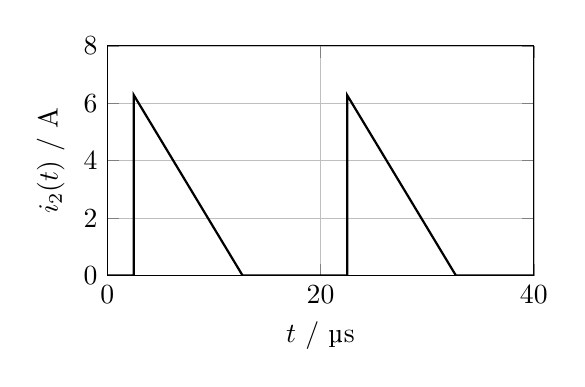
\begin{tikzpicture}
    \begin{axis}[
        width=7cm, height=4.5cm,
        grid=both,
        major grid style={line width=.2pt,draw=gray!50},
        minor grid style={line width=.1pt,draw=gray!20},
        xlabel={$t$ / µs},
        ylabel={$i_\mathrm{2}(t)$ / A},
       % title={$i_\mathrm{L}$ for minimum output power},
        xmin=0, xmax=40,
        ymin=-0, ymax=8,
        xtick={0, 20, 40},
        ytick={0, 2,4,6,8},
        ]
        % Einschaltverhalten graph
        \addplot[
            thick,
            mark=none,
            color=black,
        ] coordinates {
            (0,0) (2.5, 0) (2.5, 6.28) (12.7, 0) (22.5, 0)(22.5, 6.28) (32.7, 0) (40, 0)
        };
    \end{axis}
    \end{tikzpicture} 
    \hspace{1cm} % Abstand zwischen den beiden Diagrammen
    \caption{Display of the current $i_\mathrm{2}(t)$.}
    \label{fig:currentSecondarySidei2Task1}
    \end{solutionfigure}
\begin{solutionfigure}[htb]
    \centering
    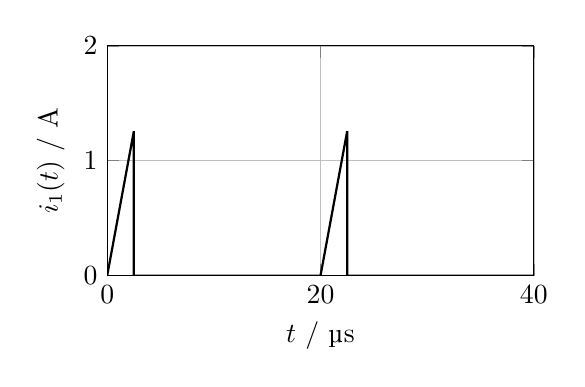
\begin{tikzpicture}
    \begin{axis}[
        width=7cm, height=4.5cm,
        grid=both,
        major grid style={line width=.2pt,draw=gray!50},
        minor grid style={line width=.1pt,draw=gray!20},
        xlabel={$t$ / µs},
        ylabel={$i_\mathrm{1}(t)$ / A},
       % title={$i_\mathrm{L}$ for minimum output power},
        xmin=0, xmax=40,
        ymin=-0, ymax=2,
        xtick={0, 20, 40},
        ytick={0, 1,2},
        ]
        % Einschaltverhalten graph
        \addplot[
            thick,
            mark=none,
            color=black,
        ] coordinates {
            (0,0) (2.5, 1.257) (2.5, 0) (20, 0)(22.5,  1.257) (22.5,  0) (40, 0)
        };
    \end{axis}
    \end{tikzpicture} 
    \hspace{1cm} % Abstand zwischen den beiden Diagrammen
    \caption{Display of the current $i_\mathrm{1}(t)$.}
    \label{fig:currentSecondarySideTask1}
    \end{solutionfigure}

\subtask{The input voltage is  $U_\mathrm{1}=\SI{382}{\volt}$ at nominal load. Determine the mean value $\overline i_\mathrm{T}$ and the effective value of the current $i_\mathrm{T, rms}$ through the transistor. Determine the mean value $\overline i_\mathrm{D}$ and the effective value of the current $i_\mathrm{D, rms}$ through the diode. What is the maximum reverse voltage load $u_\mathrm{T, max}$ of the transistor? What is the maximum reverse voltage load $u_\mathrm{D, max}$ of the diode?}
\begin{solutionblock}
    \begin{equation}
        \overline{i}_\mathrm{T} = \frac{1}{T_\mathrm{S}}\frac{1}{2}\hat I_\mathrm{1}T_\mathrm{on}=\frac{1}{\SI{20}{\micro\s}}\cdot\frac{1}{2}\SI{1.257}{\ampere}\cdot\SI{2.5}{\micro\s}=\SI{78.53}{\milli\ampere}
    \end{equation}
    \begin{equation}
        i_\mathrm{T,rms}^2=\frac{1}{T_\mathrm{S}} \int_{0}^{T_\mathrm{S}} i_\mathrm{1}^2(t) \,dt \ = \frac{1}{T_\mathrm{S}}\int_{0}^{T_\mathrm{on}} \frac{\hat I_\mathrm{1}^2t^2}{T_\mathrm{on}^2} \,dt \ =  \frac{\hat I_\mathrm{1}^2T_\mathrm{on}}{3T_\mathrm{on}}
    \end{equation}
    \begin{equation}
        i_\mathrm{T,rms} = \hat I_\mathrm{1} \sqrt{\frac{T_\mathrm{on}}{3T_\mathrm{S}}}= \SI{1.257}{\ampere}\cdot\sqrt{\frac{\SI{2.5}{\micro\s}}{3\cdot\SI{20}{\micro\s}}}= \SI{256.58}{\milli\ampere}
    \end{equation}

    \begin{equation}
        \overline{i}_\mathrm{D} = \frac{1}{T_\mathrm{S}}\frac{1}{2}\hat I_\mathrm{2}T_\mathrm{off}=\frac{1}{\SI{20}{\micro\s}}\cdot\frac{1}{2}\SI{6.28}{\ampere}\cdot\SI{12.7}{\micro\s}=\SI{2}{\ampere}
    \end{equation}

    \begin{equation}
        i_\mathrm{D,rms} = \hat I_\mathrm{2} \sqrt{\frac{T_\mathrm{off}}{3T_\mathrm{S}}}= \SI{6.28}{\ampere}\cdot\sqrt{\frac{\SI{12.7}{\micro\s}}{3\cdot\SI{20}{\micro\s}}}= \SI{2.89}{\milli\ampere}
    \end{equation}

    \begin{equation}
        u_\mathrm{T,max} = U_\mathrm{1} + \frac{N_\mathrm{1}}{N_\mathrm{2}}U_\mathrm{2}= \SI{382}{\volt}+\frac{60}{12}\cdot\SI{15}{\volt}= \SI{457}{\volt}
    \end{equation}

    \begin{equation}
        u_\mathrm{D,max} = U_\mathrm{2} + \frac{N_\mathrm{2}}{N_\mathrm{1}}U_\mathrm{1}= \SI{15}{\volt}+\frac{12}{60}\cdot\SI{382}{\volt}= \SI{91.4}{\volt}
    \end{equation}

\end{solutionblock}

\subtask{The input voltage is  $U_\mathrm{1}=\SI{382}{\volt}$ at nominal load. How much energy is transferred from the input to the output per switching period $\Delta E$ and what is the resulting average power? What happens if there is no ideal voltage source on the output side but an unloaded capacitor and the circuit is operated with $D>0$?}

\begin{solutionblock}

At each switching interval, energy is pushed into the capacitor, the voltage of which continues to rise until a component fails due to a lack of dielectric strength.    
\end{solutionblock}

%%%%%%%%%%%%%%%%%%%%%%%%%%%%%%%%%%%%%%%%%%%%%%%%%%%%%%%%%%%%%%%%%%%%%%%%%%%%%%%%%%%%%%%%%%%%%%%%%%%%%%%%%%
%% Task 2: Forward converter with asymmetric half-bridge
%%%%%%%%%%%%%%%%%%%%%%%%%%%%%%%%%%%%%%%%%%%%%%%%%%%%%%%%%%%%%%%%%%%%%%%%%%%%%%%%%%%%%%%%%%%%%%%%%%%%%%%%%%

\task{Forward converter with asymmetric half-bridge}

The schematic of a forward converter with an asymmetric half-bridge is shown in \autoref{fig:ex04_ForwardConverterWithAsymHalfBridge}. 
For the calculations the diodes and transistors are considered as ideal components.

%%%%%%%%%%%%%%%%%%%%%%%%%%%%%%%%%%%%%%%%%%%%%%%%%%%%%%%%%%%%%%%%%%%%%%%%%%
%  Forward converter with asymmetric half-bridge
%%%%%%%%%%%%%%%%%%%%%%%%%%%%%%%%%%%%%%%%%%%%%%%%%%%%%%%%%%%%%%%%%%%%%%%%%%

\begin{figure}[ht]
    \begin{center}
        \begin{circuitikz}[european currents,european resistors,american inductors]
            \draw 
                    % Base point for voltage supply
                    (0,0) coordinate (jU1v)
                    % Add supply U1
                    (jU1v) to [V=$U_1$] ++(0,-7.5) coordinate (jU1g)
                    % Add junction for Transistor TBc
                    (jU1v) to [short,-*] ++(2,0) coordinate (jTBc)
                    % Add junction for Transistor TBe
                    (jTBc) ++ (0,-2) coordinate (jTBe)
                    % Add transistor TB
                    % (jTBc) ++ (0,-1) [Tnpn, n=npn1](TB){}
                    (jTBc) ++ (0,-2) node[npn, anchor=E](TB){}
                    % At transistor label T2
                    (TB)  node[anchor=east,color=black]{$T_\mathrm{B}$}                     
                    % Connect Transistor
                    (jTBe) to [short,-] (TB.E)
                    (jTBc) to [short,-] (TB.C)
                    (TB.B) to [sqV] ++(-1,0);                    
                    % Add inductor transistor TB
                    %(jTBe) to [L,l=$L_\mathrm{T}$,n=L1,v_<=$U_\text{s}$, voltage shift=0.5, voltage=straight] (jTBc);
            \draw                    
                    % Add connection point of the diode DFP
                    (jTBe) ++(0,-3) coordinate (jDFPa)
                    % Add diode DFP
                    (jDFPa) to [D,l^=$D_\mathrm{Fp}$] (jTBe)
                    % Add connection to U1g
                    (jDFPa) to [short,-] (jU1g)
                    % Add junction for transformer Ltpv
                    (jTBc) to [short,-] ++(2,0)  coordinate  (jLtpv)
                    % Add arrow and Text
                    (jTBc) ++(1,0) node[currarrow](IP){}  
                    (IP)  node[anchor=south,color=black]{$i_\mathrm{p}$}                   
                    % Add junction for Transistor
                    (jLtpv) ++(0,-3) coordinate (jTd)
                    % Add junction for Transistor
                    (jTd) ++(0,-3) coordinate (jTs)
                    % Add transistor T2
                    (jTs) ++ (0,1.5) node[nigfete,xscale=-1](Trans1){}
                    % At transistor label T2
                    (Trans1)  node[anchor=east,color=black]{$T$}                     
                    % Connect Transistor
                    (jTs) to [short,-] (Trans1.S)
                    (jTd) to [short,-] (Trans1.D)
                    (Trans1.G) to [sqV] ++(1,0)
                    % Add connection to diode DFp
                    (jTs) to [short,-*] (jDFPa)
                    % Assign Transistor drain junction to primary junction point
                    (jTd) coordinate  (jLtpg)
                    % Add transformer primary inductor with voltage arrow
                    (jLtpv) to [L, n=Ltp, v_=$U_\text{p}$, voltage=straight] ++(0,-3) coordinate (jLtpg)
                    % Add junctions for secondary inductor
                    (jLtpv) ++(0.8,0) coordinate  (jLtsv) 
                    (jLtpg) ++(0.8,-0.5) coordinate  (jLtsgx)
                    % Add winding text
                    (jLtpg) node[left] {$N_\mathrm{p}$};         
                    % Add iron core
            \draw 
                    (jLtpv) ++(0.5,-0.5) coordinate  (jLtcorev) 
                    (jLtpg) ++(0.5,0.5) coordinate  (jLtcoreg)
                    (jLtcorev) to [short, double, double distance=3pt, thick]  (jLtcoreg)
                    let \p1 = (jLtcorev), \p2 = (jLtcoreg) in [double, double distance=3pt, thick]
                    (\x1/2+\x2/2, \y1) -- (\x1/2+\x2/2, \y2); 
            \draw 
                    % Add transformer secondary inductor with voltage arrow
                    (jLtsv) to [L,n=Lts,v^=$U_\text{s}$, voltage shift=0.5, voltage=straight] ++(0,-3) coordinate (jLtsg)
                    % Add winding text
                    (jLtsg) node[right] {$N_\mathrm{s}$};     
                    \path (Ltp.ul dot) node[circ]{};
                    \path (Lts.ul dot) node[circ]{};                    
            \draw
                    % Add arrow and Text
                    (jLtsv) ++(0.5,0) node[currarrow](IS){}  
                    (IS)  node[anchor=south,color=black]{$i_\mathrm{s}$}
                     % Add D1
                    (jLtsv) to  [D,l^=$D_1$] ++ (2,0) coordinate (jD1k)
                    % Add junction point for DFsk
                    (jD1k)  to [short,-*] ++(0,0) coordinate (jDFsk)
                    % Add junction point for DFsa
                    (jDFsk)  ++ (0,-3.5) coordinate (jDFsa)
                    % Add diode DFs
                    (jDFsa) to  [D,l^=$D_\mathrm{Fs}$]  (jDFsk)                    
                    % Add inductor L
                    (jDFsk) to [L,l=$L$,n=L1] ++(3,0) coordinate (jU2v)
                    % Add arrow and Text
                    (jDFsk) ++(0.5,0) node[currarrow](IL){}  
                    (IL)  node[anchor=south,color=black]{$i_\mathrm{L}$}
                    % Add output voltage U2
                    (jU2v) to [V=$U_2$] ++(0,-3.5) coordinate (jU2g)
                    % Add connection to DFs
                    (jU2g) to [short,-*] (jDFsa)
                    % Add connection to LTsgx
                    (jDFsa) to [short,-] (jLtsgx)
                    % Add connection to LTsgx
                    (jLtsgx) to [short,-] (jLtsg);

                \end{circuitikz}
    \end{center}
    \caption{Forward converter with asymmetric half-bridge.}
    \label{fig:ex04_ForwardConverterWithAsymHalfBridge}
\end{figure}


The parameters are listed in \autoref{fig:ex04_ForwardConverterWithAsymHalfBridge}.

%%%%%%%%%%%%%%%%%%%%%%%%%%%%%%%%%%%%%%%%%%%%%%%%%%%%%%%%%%%%%%%%%%%%%%%%%%
%  Parameter of the forward converter with asymmetric half-bridge
%%%%%%%%%%%%%%%%%%%%%%%%%%%%%%%%%%%%%%%%%%%%%%%%%%%%%%%%%%%%%%%%%%%%%%%%%%

\begin{table}[htb]
    \centering  % Zentriert die Tabelle
    \begin{tabular}{llll}
        \toprule
        Input voltage: &  $U_{\mathrm{1}} = \SI{325}{\volt}$ & Output voltage: & $U_{\mathrm{2}} = \SI{15}{\volt}$ \\ 
        Output power: & $P_{\mathrm{2}} = \SI{50}{\watt}$ & Switching frequency: & $f_{\mathrm{s}} = \SI{50}{\kilo\hertz}$ \\
        Turns ration: &  $N_{\mathrm{1}}/N_{\mathrm{2}}=10$ & Magnetizing inductance: & $L_{\mathrm{m}}=\SI{2}{\milli\henry}$  \\
        \bottomrule
    \end{tabular}
    \caption{Parameter overview of the circuit.}
    \label{table:Ex04_Forward converter with asymmetric half-bridge}
\end{table}
\FloatBarrier
The leakage inductance, the resistive losses, and the core losses of the transformer are negligible. 
The converter operates in steady-state conditions. Both transistors are controlled by the same signal.

\subtask{At what duty cycle $D$ does the circuit operate?}
\subtask{Calculate the average value of $\overline{i_\mathrm{2}}$ and $\overline{i_\mathrm{1}}$ over a switching cycle, 
         assuming ideal filtering of $i_\mathrm{2}$.}
\subtask{Calculate the peak value of $\hat{i}_\mathrm{m}$ the magnetizing current $i_\mathrm{m}$.}
\subtask{Sketch the waveforms of $u_\mathrm{p}$, $i_\mathrm{m}$, $i_\mathrm{p}$ and $i_\mathrm{1}$ 
         considering switching-induced ripples.}
\subtask{Calculate the minimal necessary input voltage $U_\mathrm{1}$, if the output voltage $U_\mathrm{2}$ = \SI{20}{\volt} shall being constant.}
\subtask{Calculate the inductance of $L$,such that the ripple current $\Delta i_\mathrm{2}$ is to be $\SI{10}{\percent}$ of the 
         average output current $\overline{I_\mathrm{2}}$?}



%%%%%%%%%%%%%%%%%%%%%%%%%%%%%%%%%%%%%%%%%%%%%%%%%%%%%%%%%%%%%%%%%%%%%%%%%%%%%%%%%%%%%%%%%%%%%%%%%%%%%%%%%%
%% Task 3: Singled-ended forward converter (demagnetization winding)
%%%%%%%%%%%%%%%%%%%%%%%%%%%%%%%%%%%%%%%%%%%%%%%%%%%%%%%%%%%%%%%%%%%%%%%%%%%%%%%%%%%%%%%%%%%%%%%%%%%%%%%%%%

\task{Singled-ended forward converter (demagnetization winding)}

The power supply of a data processing system shall be realized by a singled-ended forward converter as shown in \autoref{fig:ex04_SingledEndedForwardConverter}.


%%%%%%%%%%%%%%%%%%%%%%%%%%%%%%%%%%%%%%%%%%%%%%%%%%%%%%%%%%%%%%%%%%%%%%%%%%
%  Single Ended Forward Converter
%%%%%%%%%%%%%%%%%%%%%%%%%%%%%%%%%%%%%%%%%%%%%%%%%%%%%%%%%%%%%%%%%%%%%%%%%%

\begin{figure}[ht]
    \begin{center}
        \begin{circuitikz}[european currents,european resistors,american inductors]
            \draw 
                    % Base point for voltage supply
                    (0,0) coordinate (jU1v)
                    % Add supply U1
                    (jU1v) to [V=$U_\mathrm{1}$] ++(0,-4) coordinate (jU1g)
                     % Add junction for inductor LT
                    (jU1v) to [short,-*] ++(2,0) coordinate (jLTv)
                    % Add junction for diode D3
                    (jLTv) ++ (0,-2) coordinate (jD3k)
                    % Add inductor LTv
                    (jD3k) to [L,l=$N_\mathrm{3}$,n=L1,v_<=$U_\mathrm{3}$, voltage shift=0.5, voltage=straight] (jLTv);
                    \path (L1.ul dot) node[circ]{};
            \draw                    
                    % Add arrow and Text
                    (jD3k) ++(0,-0.5) node[currarrow,rotate=90](IT){}  
                    (IT)  node[anchor=east,color=black]{$i_\mathrm{3}$}
                    % Add connection point of the diode D3
                    (jD3k) ++(0,-2) coordinate (jD3a)
                    % Add diode D3
                    (jD3a) to [D,l^=$D_\mathrm{3}$] (jD3k)
                    % Add connection to U1g
                    (jD3a) to [short,-] (jU1g)
                    % Add junction for transformer Ltpv
                    (jLTv) to [short,-] ++(2.5,0)  coordinate  (jLtpv)
                    % Add arrow and Text
                    (jLTv) ++(1,0) node[currarrow](IP){}  
                    (IP)  node[anchor=south,color=black]{$i_\mathrm{p}$}                   
                    % Add junction for Transistor
                    (jLtpv) ++(0,-2) coordinate (jTd)
                    % Add junction for Transistor
                    (jTd) ++(0,-2) coordinate (jTs)
                    % Add transistor T2
                    (jTs) ++ (0,1) node[nigfete,xscale=-1](Trans1){}
                    % At transistor label T2
                    (Trans1)  node[anchor=east,color=black]{$T$}                     
                    % Connect Transistor
                    (jTs) to [short,-] (Trans1.S)
                    (jTd) to [short,-] (Trans1.D)
                    (Trans1.G) to [sqV] ++(1,0)
                    % Add connection to diode D3
                    (jTs) to [short,-*] (jD3a)
                    % Assign Transistor drain junction to primary junction point
                    (jTd) coordinate  (jLtpg)
                    % Add transformer primary inductor with voltage arrow
                    (jLtpv) to [L,l_=$N_\mathrm{1}$, n=Ltp, v_=$U_\mathrm{p}$,voltage shift=5, voltage=straight] ++(0,-2) coordinate (jLtpg)
                    % Add junctions for secondary inductor
                    (jLtpv) ++(0.8,0) coordinate  (jLtsv) 
                    (jLtpg) ++(0.8,0) coordinate  (jLtsg);      
                    % Add iron core
            \draw 
                    (jLtpv) ++(0.4,-0.5) coordinate  (jLtcorev) 
                    (jLtpg) ++(0.4,0.5) coordinate  (jLtcoreg)
                    (jLtcorev) to [short, double, double distance=3pt, thick]  (jLtcoreg)
                    let \p1 = (jLtcorev), \p2 = (jLtcoreg) in [double, double distance=3pt, thick]
                    (\x1/2+\x2/2, \y1) -- (\x1/2+\x2/2, \y2); 
            \draw 
                    % Add transformer secondary inductor with voltage arrow
                    (jLtsv) to [L,l^=$N_\mathrm{2}$,n=Lts,mirror,v^=$U_\mathrm{s}$, voltage shift=5, voltage=straight] (jLtsg);
                    \path (Ltp.ul dot) node[circ]{};
                    \path (Lts.ul dot) node[circ]{};                    
            \draw
                    % Add arrow and Text
                    (jLtsv) ++(0.5,0) node[currarrow](IS){}  
                    (IS)  node[anchor=south,color=black]{$i_\mathrm{s}$}
                     % Add D1
                    (jLtsv) to  [D,l^=$D_\mathrm{1}$] ++ (3,0) coordinate (jD1k)
                    % Add junction point for D2k
                    (jD1k)  to [short,-*] ++(0,0) coordinate (jD2k)
                    % Add junction point for D2a
                    (jD2k)  ++ (0,-2) coordinate (jD2a)
                    % Add diode D2
                    (jD2a) to  [D,l^=$D_\mathrm{2}$]  (jD2k)                    
                    % Add inductor L4
                    (jD2k) to [L,l=$L$,n=L1] ++(3,0) coordinate (jU2v)
                    % Add arrow and Text
                    (jD2k) ++(0.5,0) node[currarrow](IL){}  
                    (IL)  node[anchor=south,color=black]{$i_\mathrm{L}$}
                    % Add output voltage U2
                    (jU2v) to [V=$U_\mathrm{2}$] ++(0,-2) coordinate (jU2g)
                    % Add connection to D2
                    (jU2g) to [short,-*] (jD2a)
                    % Add connection to secondary transformer LTsg
                    (jD2a) to [short,-] (jLtsg);

                \end{circuitikz}
    \end{center}
    \caption{Single ended forward converter circuit.}
    \label{fig:ex04_SingledEndedForwardConverter}
\end{figure}


The parameters are listed in \autoref{table:Ex04_Parameters of the singled ended forward converter.}.
The output inductance is dimensioned so that the current $i_\mathrm{L}$ exhibits a continuous waveform.
The transformer's leakage inductance can be neglected.

%%%%%%%%%%%%%%%%%%%%%%%%%%%%%%%%%%%%%%%%%%%%%%%%%%%%%%%%%%%%%%%%%%%%%%%%%%
%  Parameter of the singled ended forward converter
%%%%%%%%%%%%%%%%%%%%%%%%%%%%%%%%%%%%%%%%%%%%%%%%%%%%%%%%%%%%%%%%%%%%%%%%%%

\begin{table}[htb]
    \centering  % Zentriert die Tabelle
    \begin{tabular}{llll}
        \toprule
        Input voltage: &  $U_{\mathrm{1}} = \SI{325}{\volt}$ & Output voltage: & $U_{\mathrm{2}} = \SI{5}{\volt}$ \\ 
        Output power: & $P_{\mathrm{2}} = \SI{125}{\watt}$ & Switching frequency: & $f_{\mathrm{s}} = \SI{48}{\kilo\hertz}$ \\
        Forward voltage of $D_{\mathrm{1}}$: & $U_{\mathrm{D1,f}} = \SI{0.4}{\volt}$ & Forward voltage of $D_{\mathrm{2}}$: & $U_{\mathrm{D2,f}} = \SI{0}{\volt}$  \\
        \bottomrule
    \end{tabular}
    \caption{Parameters of the circuit.}  % Beschriftung der Tabelle
    \label{table:Ex04_Parameters of the singled ended forward converter.}
\end{table}

\subtask{Calculate the turns ratio $N_\mathrm{3}$/$N_\mathrm{1}$ so that the maximum blocking voltage 
         across the transistor during demagnetization is $\SI{600}{\volt}$.}
\subtask{What is the maximum permissible duty cycle of the power transistor in this case?}
\subtask{What turns ratio $N_\mathrm{1}$/$N_\mathrm{2}$ should be chosen to achieve the required secondary voltage?}
\subtask{Does the steady-state duty cycle of the transistor need to be adjusted when the output power changes? 
         Over what range must the transistor's duty cycle be adjustable, considering the input voltage range?}
\subtask{What are the resulting maximum blocking voltages of the diodes $D_\mathrm{1}$ and $D_\mathrm{2}$?}
\subtask{What should be the value of the primary inductance $L_\mathrm{1}$ to ensure 
        that the peak value of the magnetizing current remains below $\SI{10}{\percent}$ of the current $\overline{i_\mathrm{L'}}$. 
        The current $\overline{i_\mathrm{L'}}$  corresponds to the average current $\overline{i_\mathrm{L}}$ through the output inductance 
        at a nominal load of $P_2=\SI{125}{\watt}$, which is translated to the primary side.}
\subtask{Sketch the waveform of the voltage across the power transistor, the current through the demagnetization 
        winding, and the current through the freewheeling diode $D_\mathrm{2}$ 
        for $U_\mathrm{1}=\SI{240}{\volt}$ and $U_\mathrm{1}=\SI{360}{\volt}$.}
\subtask{Calculate the peak value of the magnetizing current for each case. Consider the current in the output 
          inductor as ideally filtered.}
\subtask{Could a higher power be transferred by doubling the switching frequency of the converter?}